\documentclass{article}\usepackage[]{graphicx}\usepackage[]{color}
%% maxwidth is the original width if it is less than linewidth
%% otherwise use linewidth (to make sure the graphics do not exceed the margin)
\makeatletter
\def\maxwidth{ %
  \ifdim\Gin@nat@width>\linewidth
    \linewidth
  \else
    \Gin@nat@width
  \fi
}
\makeatother

\definecolor{fgcolor}{rgb}{0.345, 0.345, 0.345}
\newcommand{\hlnum}[1]{\textcolor[rgb]{0.686,0.059,0.569}{#1}}%
\newcommand{\hlstr}[1]{\textcolor[rgb]{0.192,0.494,0.8}{#1}}%
\newcommand{\hlcom}[1]{\textcolor[rgb]{0.678,0.584,0.686}{\textit{#1}}}%
\newcommand{\hlopt}[1]{\textcolor[rgb]{0,0,0}{#1}}%
\newcommand{\hlstd}[1]{\textcolor[rgb]{0.345,0.345,0.345}{#1}}%
\newcommand{\hlkwa}[1]{\textcolor[rgb]{0.161,0.373,0.58}{\textbf{#1}}}%
\newcommand{\hlkwb}[1]{\textcolor[rgb]{0.69,0.353,0.396}{#1}}%
\newcommand{\hlkwc}[1]{\textcolor[rgb]{0.333,0.667,0.333}{#1}}%
\newcommand{\hlkwd}[1]{\textcolor[rgb]{0.737,0.353,0.396}{\textbf{#1}}}%

\usepackage{framed}
\makeatletter
\newenvironment{kframe}{%
 \def\at@end@of@kframe{}%
 \ifinner\ifhmode%
  \def\at@end@of@kframe{\end{minipage}}%
  \begin{minipage}{\columnwidth}%
 \fi\fi%
 \def\FrameCommand##1{\hskip\@totalleftmargin \hskip-\fboxsep
 \colorbox{shadecolor}{##1}\hskip-\fboxsep
     % There is no \\@totalrightmargin, so:
     \hskip-\linewidth \hskip-\@totalleftmargin \hskip\columnwidth}%
 \MakeFramed {\advance\hsize-\width
   \@totalleftmargin\z@ \linewidth\hsize
   \@setminipage}}%
 {\par\unskip\endMakeFramed%
 \at@end@of@kframe}
\makeatother

\definecolor{shadecolor}{rgb}{.97, .97, .97}
\definecolor{messagecolor}{rgb}{0, 0, 0}
\definecolor{warningcolor}{rgb}{1, 0, 1}
\definecolor{errorcolor}{rgb}{1, 0, 0}
\newenvironment{knitrout}{}{} % an empty environment to be redefined in TeX

\usepackage{alltt}
\usepackage{fullpage}
\usepackage{placeins}
\usepackage[colorlinks=true, linkcolor=blue]{hyperref}
\title{Lab 2 Pattern Analysis-First Order Effect}
\author{Dominic LaRoche}
\IfFileExists{upquote.sty}{\usepackage{upquote}}{}
\begin{document}
\maketitle
For this lab we use the Japanese black pine sapling data which is dscribed below.
\begin{knitrout}
\definecolor{shadecolor}{rgb}{0.969, 0.969, 0.969}\color{fgcolor}\begin{kframe}
\begin{alltt}
\hlkwd{rm}\hlstd{(}\hlkwc{list}\hlstd{=}\hlkwd{ls}\hlstd{())}
\hlkwd{library}\hlstd{(spatstat)}
\end{alltt}


{\ttfamily\noindent\itshape\color{messagecolor}{\#\# \\\#\# spatstat 1.38-1\ \ \ \ \ \  (nickname: 'Le Hardi') \\\#\# For an introduction to spatstat, type 'beginner'}}\begin{alltt}
\hlkwd{data}\hlstd{(japanesepines)}
\hlstd{jp}\hlkwb{<-}\hlstd{japanesepines}
\hlkwd{class}\hlstd{(jp)}
\end{alltt}
\begin{verbatim}
## [1] "ppp"
\end{verbatim}
\end{kframe}
\end{knitrout}


\begin{knitrout}
\definecolor{shadecolor}{rgb}{0.969, 0.969, 0.969}\color{fgcolor}\begin{kframe}
\begin{alltt}
\hlkwd{summary}\hlstd{(jp)}
\end{alltt}
\begin{verbatim}
## Planar point pattern:  65 points
## Average intensity 65 points per square unit (one unit = 5.7 metres)
## 
## Coordinates are given to 2 decimal places
## i.e. rounded to the nearest multiple of 0.01 units (one unit = 5.7 metres)
## 
## Window: rectangle = [0, 1] x [0, 1] units
## Window area = 1 square unit
## Unit of length: 5.7 metres
\end{verbatim}
\begin{alltt}
\hlkwd{par}\hlstd{(}\hlkwc{xpd}\hlstd{=T)}
\hlkwd{plot}\hlstd{(jp,}\hlkwc{axes}\hlstd{=T,} \hlkwc{main}\hlstd{=}\hlstr{"Japanese black pine saplings"}\hlstd{)}
\end{alltt}
\end{kframe}
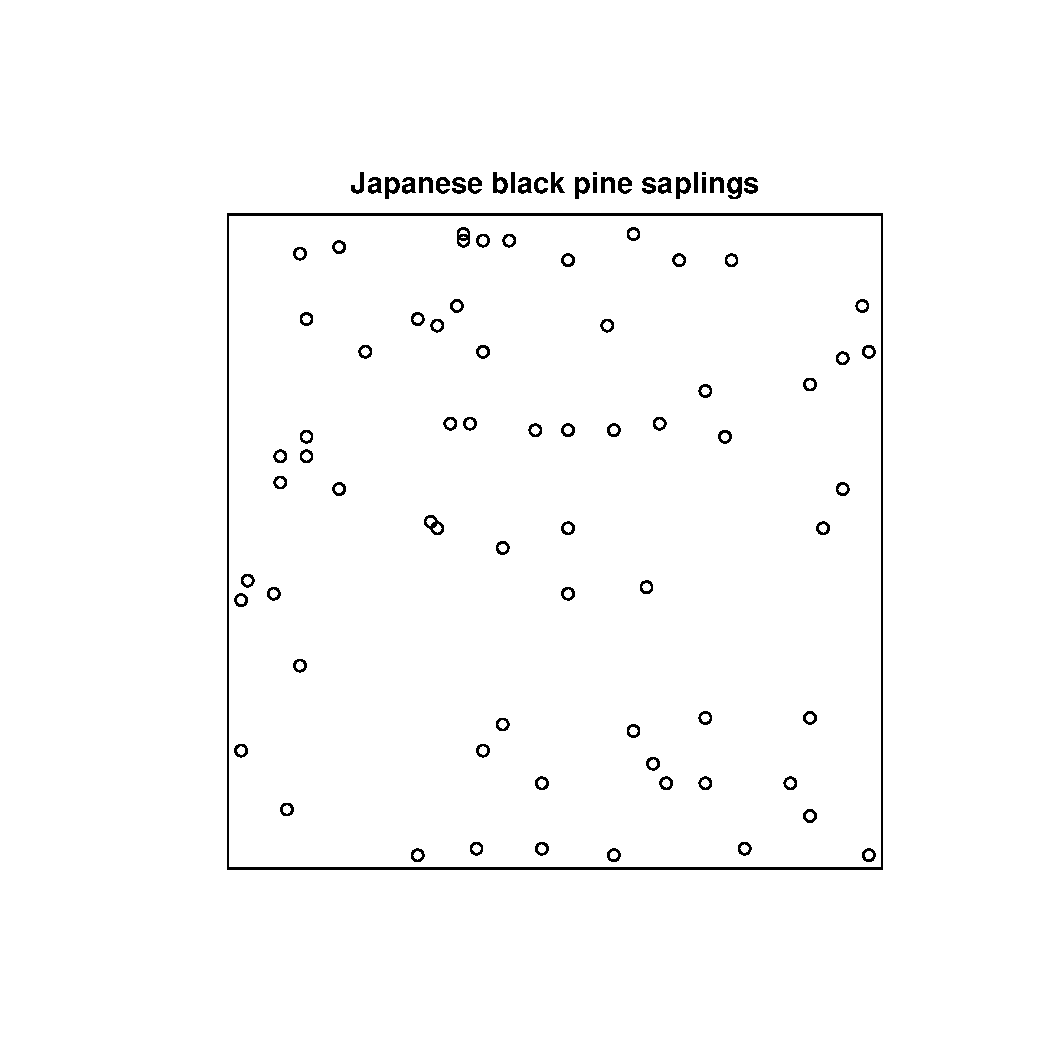
\includegraphics[width=\maxwidth]{figure/Summarize} 

\end{knitrout}



\FloatBarrier
\section{Assignment I: Quadrat Tests}
We will test for a first order effect using two different quadrat tests, one with 4 cells (2x2) and one with 16 (4x4).  The two grids are shown in figure~\ref{quads}.\\

\begin{figure}
\begin{knitrout}
\definecolor{shadecolor}{rgb}{0.969, 0.969, 0.969}\color{fgcolor}\begin{kframe}
\begin{alltt}
\hlkwd{par}\hlstd{(}\hlkwc{mfrow}\hlstd{=}\hlkwd{c}\hlstd{(}\hlnum{1}\hlstd{,}\hlnum{2}\hlstd{))}
\hlcom{#2x2}
\hlstd{q.jp2}\hlkwb{<-}\hlkwd{quadratcount}\hlstd{(jp,}\hlkwc{nx}\hlstd{=}\hlnum{2}\hlstd{,}\hlkwc{ny}\hlstd{=}\hlnum{2}\hlstd{)}
\hlkwd{plot} \hlstd{(jp,} \hlkwc{pch}\hlstd{=}\hlstr{"+"}\hlstd{,} \hlkwc{main} \hlstd{=} \hlstr{" 2x2 Quadrat for jp data"}\hlstd{)}
\hlkwd{plot} \hlstd{(q.jp2,} \hlkwc{add}\hlstd{=}\hlnum{TRUE}\hlstd{,} \hlkwc{col}\hlstd{=}\hlstr{"red"}\hlstd{,} \hlkwc{cex}\hlstd{=}\hlnum{1.5}\hlstd{,} \hlkwc{lty}\hlstd{=}\hlnum{2}\hlstd{)}
\hlcom{#4x4}
\hlstd{q.jp4}\hlkwb{<-}\hlkwd{quadratcount}\hlstd{(jp,}\hlkwc{nx}\hlstd{=}\hlnum{4}\hlstd{,}\hlkwc{ny}\hlstd{=}\hlnum{4}\hlstd{)}
\hlkwd{plot} \hlstd{(jp,} \hlkwc{pch}\hlstd{=}\hlstr{"+"}\hlstd{,} \hlkwc{main} \hlstd{=} \hlstr{"4x4 Quadrat for jp data"}\hlstd{)}
\hlkwd{plot} \hlstd{(q.jp4,} \hlkwc{add}\hlstd{=}\hlnum{TRUE}\hlstd{,} \hlkwc{col}\hlstd{=}\hlstr{"red"}\hlstd{,} \hlkwc{cex}\hlstd{=}\hlnum{1.5}\hlstd{,} \hlkwc{lty}\hlstd{=}\hlnum{2}\hlstd{)}
\end{alltt}
\end{kframe}
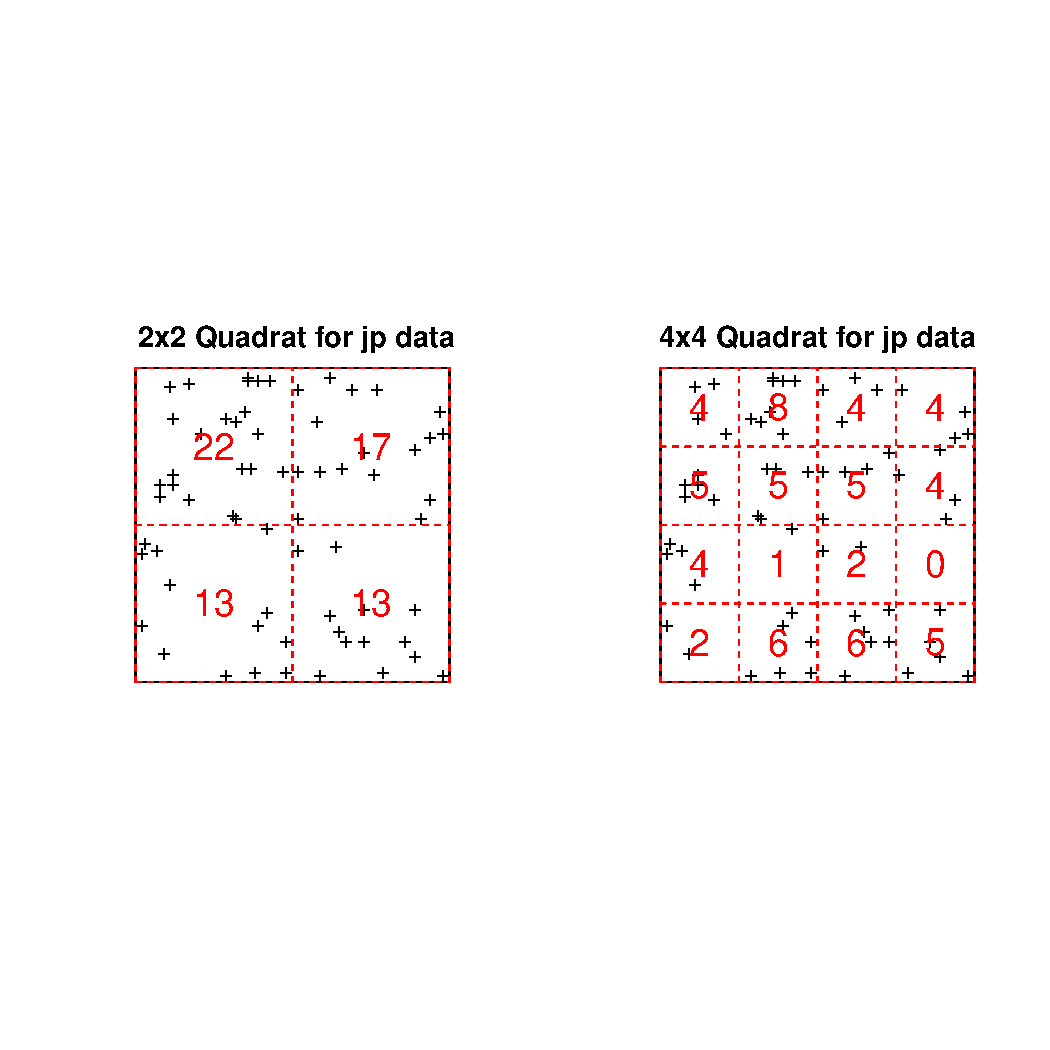
\includegraphics[width=\maxwidth]{figure/FirstOrderEffect} 

\end{knitrout}
\caption{Quadrat counts for the Japanese black pine data.}
\label{quads}
\end{figure}

We cannot reject the null hypothesis of complete spatial randomness with either the 2x2 or 4x4 quadrat tests ($\alpha \leq 0.1$).  However, the test statistic was highly dependent on the number of quadrats selected (the 3x3 test was nearly significant), which is not a desireable property. Moreover, Figures ~\ref{qt.jp2} and ~\ref{qt.jp4} show the counts and expected values for each cell.\\
\begin{knitrout}
\definecolor{shadecolor}{rgb}{0.969, 0.969, 0.969}\color{fgcolor}\begin{kframe}
\begin{alltt}
\hlstd{qt.jp2}\hlkwb{<-}\hlkwd{quadrat.test}\hlstd{(jp,}\hlnum{2}\hlstd{,}\hlnum{2}\hlstd{)}
\hlstd{qt.jp2}
\end{alltt}
\begin{verbatim}
## 
## 	Chi-squared test of CSR using quadrat counts
## 	Pearson X2 statistic
## 
## data:  jp
## X2 = 3.369, df = 3, p-value = 0.6762
## alternative hypothesis: two.sided
## 
## Quadrats: 2 by 2 grid of tiles
\end{verbatim}
\begin{alltt}
\hlstd{qt.jp4}\hlkwb{<-}\hlkwd{quadrat.test}\hlstd{(jp,}\hlnum{4}\hlstd{,}\hlnum{4}\hlstd{)}
\end{alltt}


{\ttfamily\noindent\color{warningcolor}{\#\# Warning: Some expected counts are small; chi\textasciicircum{}2 approximation may be inaccurate}}\begin{alltt}
\hlstd{qt.jp4}
\end{alltt}
\begin{verbatim}
## 
## 	Chi-squared test of CSR using quadrat counts
## 	Pearson X2 statistic
## 
## data:  jp
## X2 = 15, df = 15, p-value = 0.9028
## alternative hypothesis: two.sided
## 
## Quadrats: 4 by 4 grid of tiles
\end{verbatim}
\end{kframe}
\end{knitrout}

\begin{figure}
\begin{knitrout}
\definecolor{shadecolor}{rgb}{0.969, 0.969, 0.969}\color{fgcolor}\begin{kframe}
\begin{alltt}
\hlkwd{plot}\hlstd{(qt.jp2,} \hlkwc{main}\hlstd{=}\hlstr{"Quadrat Test: 2x2 JP data"}\hlstd{)}
\hlkwd{plot}\hlstd{(jp,} \hlkwc{pch}\hlstd{=}\hlstr{"+"}\hlstd{,} \hlkwc{col}\hlstd{=}\hlstr{"red"}\hlstd{,} \hlkwc{add}\hlstd{=T)}
\end{alltt}
\end{kframe}
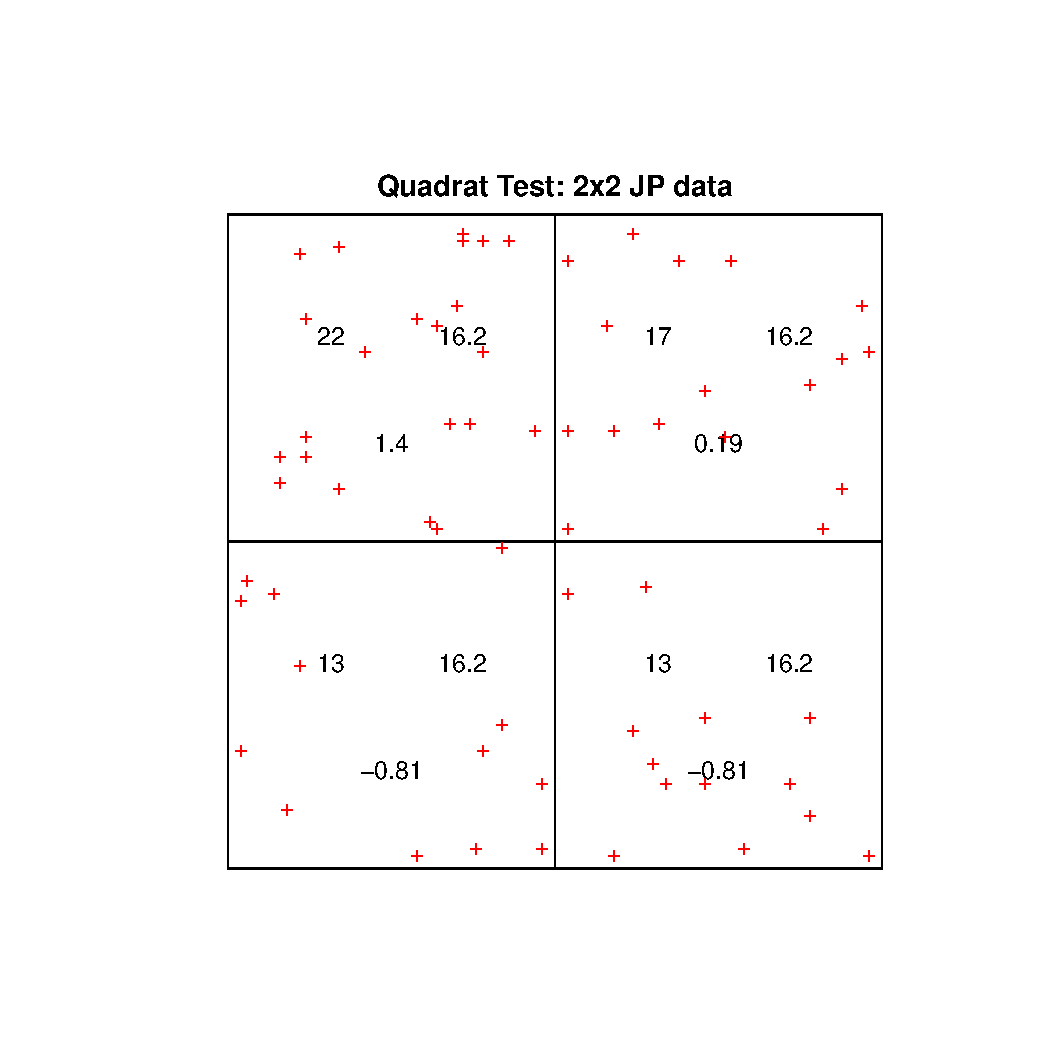
\includegraphics[width=\maxwidth]{figure/plottests2x2} 

\end{knitrout}
\caption{A plot of the test for the 2x2 quadrat test.}
\label{qt.jp2}
\end{figure}

\begin{figure}
\begin{knitrout}
\definecolor{shadecolor}{rgb}{0.969, 0.969, 0.969}\color{fgcolor}\begin{kframe}
\begin{alltt}
\hlkwd{plot}\hlstd{(qt.jp4,} \hlkwc{main}\hlstd{=}\hlstr{"Quadrat Test: 4x4 JP data"}\hlstd{)}
\hlkwd{plot}\hlstd{(jp,} \hlkwc{pch}\hlstd{=}\hlstr{"+"}\hlstd{,} \hlkwc{col}\hlstd{=}\hlstr{"red"}\hlstd{,} \hlkwc{add}\hlstd{=T)}
\end{alltt}
\end{kframe}
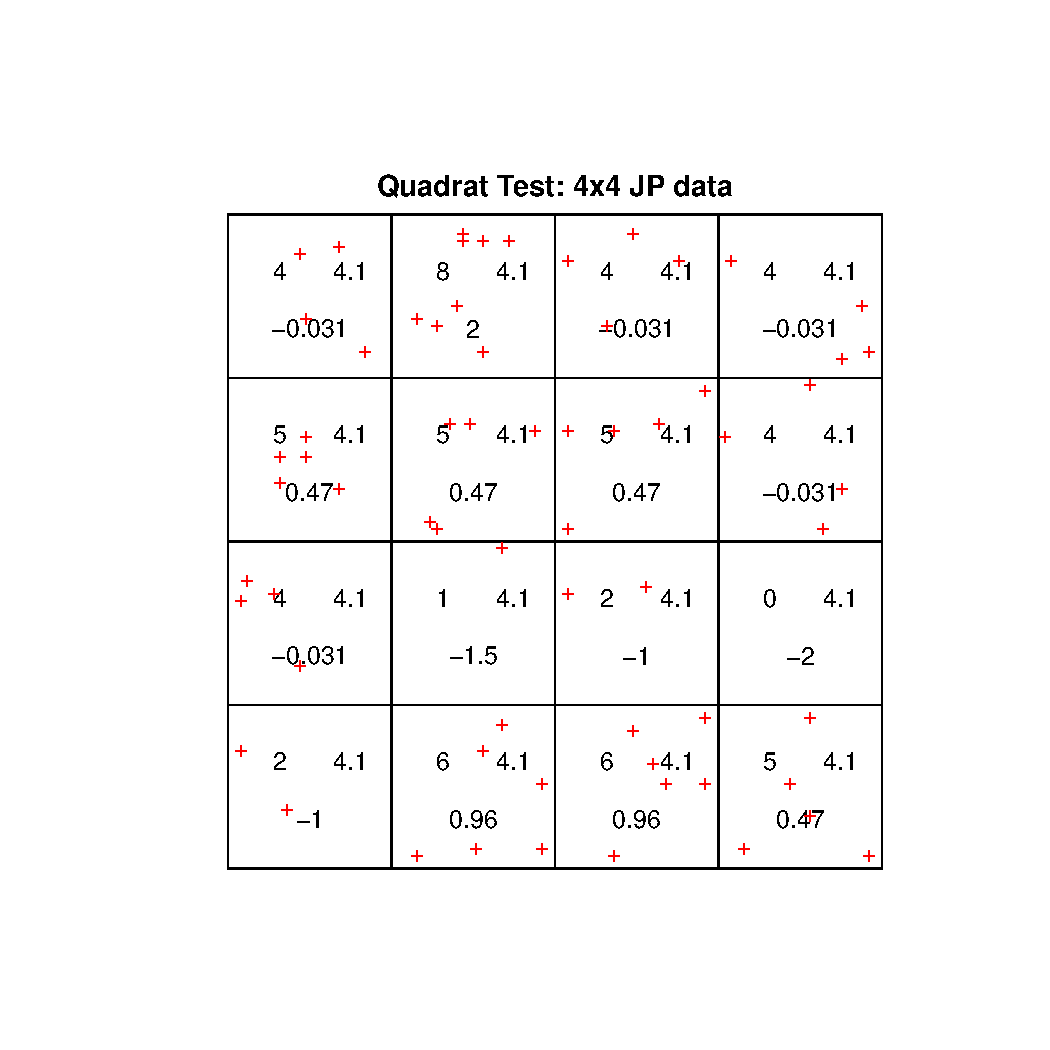
\includegraphics[width=\maxwidth]{figure/plottests4x4} 

\end{knitrout}
\caption{A plot of the test for the 4x4 quadrat test.}
\label{qt.jp4}
\end{figure}
\FloatBarrier

\section{Assignment II: Kernel estimation}
Kernel estimation is subject to the bandwidth selected by the user.  Figure~\ref{kern} shows two different realizations of kernel density estimation with bandwidths equal to 0.05 (top) and 0.1 (bottom).  The smaller bandwith gives a much closer fit to the actual points but this may not approximate the underlying process very well.  The larger bandwidth may over smooth the underlying density and hide real patterns.\\
\begin{figure}
\begin{knitrout}
\definecolor{shadecolor}{rgb}{0.969, 0.969, 0.969}\color{fgcolor}\begin{kframe}
\begin{alltt}
\hlcom{# ?density.ppp}
\hlkwd{par}\hlstd{(}\hlkwc{mfrow}\hlstd{=}\hlkwd{c}\hlstd{(}\hlnum{2}\hlstd{,}\hlnum{1}\hlstd{))}
\hlstd{jp.Z.0.5}\hlkwb{<-}\hlkwd{density.ppp}\hlstd{(jp,} \hlnum{0.05}\hlstd{)}
\hlkwd{plot}\hlstd{(jp.Z.0.5,} \hlkwc{main}\hlstd{=}\hlstr{"Kernel Estimation of JP: sigma=0.05"}\hlstd{)}
\hlkwd{points}\hlstd{(jp,} \hlkwc{pch}\hlstd{=}\hlstr{"+"}\hlstd{,} \hlkwc{col}\hlstd{=}\hlstr{"6"}\hlstd{)}

\hlstd{jp.Z.1}\hlkwb{<-}\hlkwd{density.ppp}\hlstd{(jp,} \hlnum{0.1}\hlstd{)}
\hlkwd{plot}\hlstd{(jp.Z.1,} \hlkwc{main}\hlstd{=}\hlstr{"Kernel Estimation of JP: sigma =0.1"}\hlstd{)}
\hlkwd{points}\hlstd{(jp,} \hlkwc{pch}\hlstd{=}\hlstr{"+"}\hlstd{,} \hlkwc{col}\hlstd{=}\hlstr{"6"}\hlstd{)}
\end{alltt}
\end{kframe}
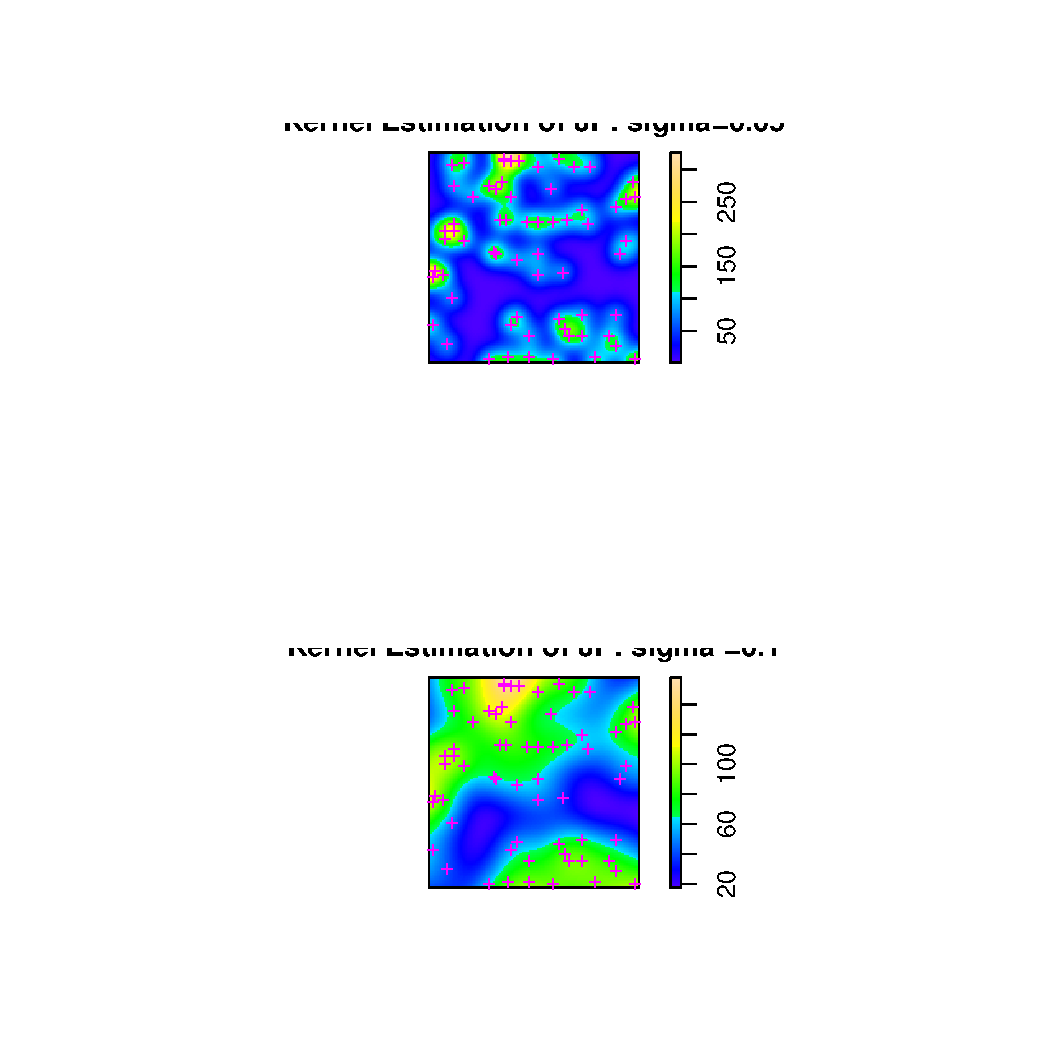
\includegraphics[width=\maxwidth]{figure/kernelest05} 

\end{knitrout}
\caption{Two different kernel density estimation with sigma =0.05 and 0.1.}
\label{kern}
\end{figure}
\FloatBarrier

\section{Assignemnt 3: Second Order Effect}
The plots of $\hat{G}$ (fig.~\ref{gest}) and $\hat{F}$ (fig.~\ref{fest}) both suggest that the pattern is random since there are no serious deviations between the theoretical and observed distances.  The $\hat{K}$ function plot (fig.~\ref{kest}) and the $\hat{L}$ function both suggest slight evidence of a regular pattern but the significance of this cannot be ascertained from the plots without confidence bands.\\

\begin{figure}
\begin{knitrout}
\definecolor{shadecolor}{rgb}{0.969, 0.969, 0.969}\color{fgcolor}\begin{kframe}
\begin{alltt}
\hlstd{jp.ghat}\hlkwb{<-}\hlkwd{Gest}\hlstd{(jp)}
\hlstd{g.max}\hlkwb{<-}\hlkwd{max}\hlstd{(jp.ghat}\hlopt{$}\hlstd{r)}
\hlkwd{plot}\hlstd{(jp.ghat,} \hlkwd{cbind}\hlstd{(rs, theo)}\hlopt{~}\hlstd{r,} \hlkwc{main}\hlstd{=}\hlstr{"G estimates"}\hlstd{,} \hlkwc{xlab}\hlstd{=}\hlstr{"Dist"}\hlstd{)}
\end{alltt}
\end{kframe}
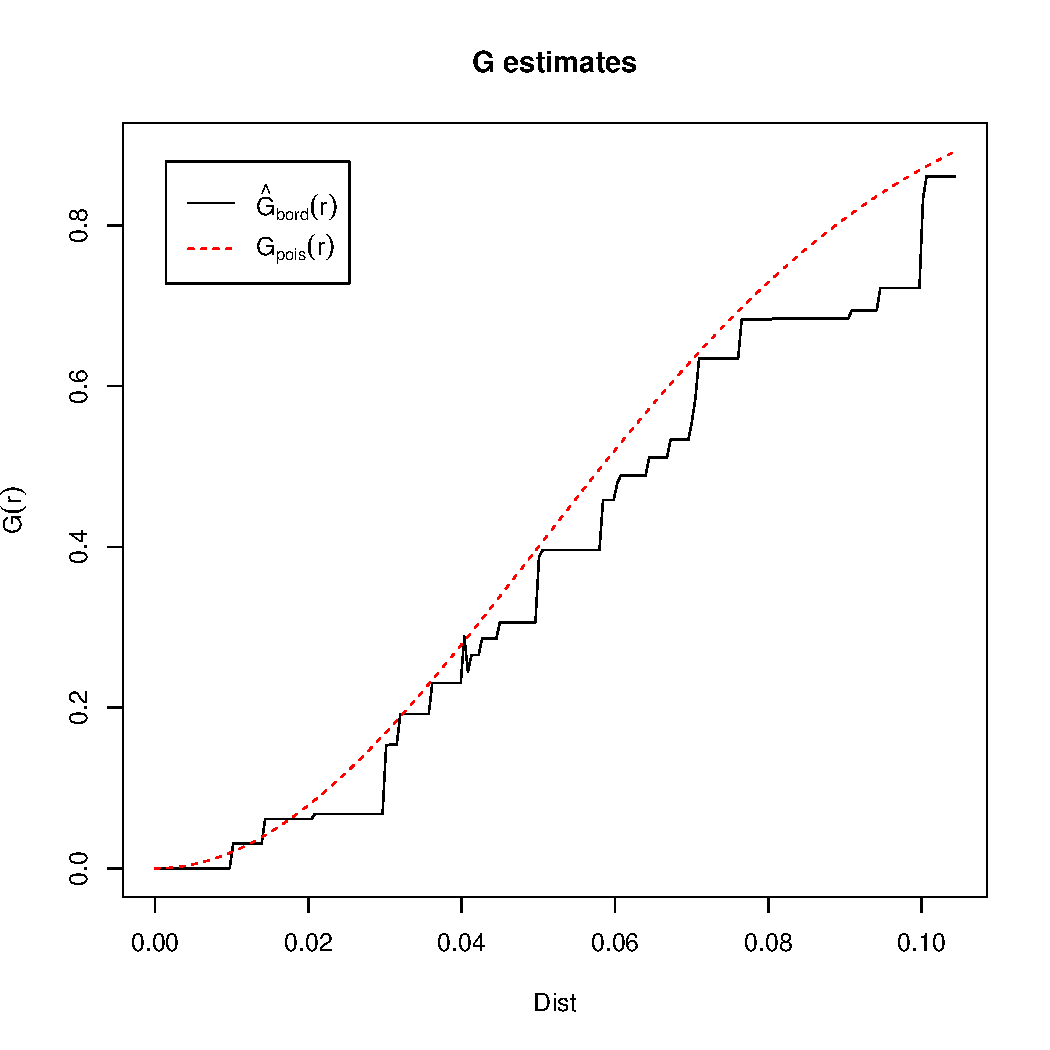
\includegraphics[width=\maxwidth]{figure/secondorder} 
\begin{kframe}\begin{verbatim}
##      lty col  key           label                           meaning
## rs     1   1   rs hat(G)[bord](r) border corrected estimate of G(r)
## theo   2   2 theo      G[pois](r)          theoretical Poisson G(r)
\end{verbatim}
\end{kframe}
\end{knitrout}
\caption{Estimation of the G function using nearest neighbor distances and comparison with a theoretical poisson distribtion.}
\label{gest}
\end{figure}

\begin{figure}
\begin{knitrout}
\definecolor{shadecolor}{rgb}{0.969, 0.969, 0.969}\color{fgcolor}\begin{kframe}
\begin{alltt}
\hlstd{jp.fhat}\hlkwb{<-}\hlkwd{Fest}\hlstd{(jp)}
\hlstd{f.max}\hlkwb{<-}\hlkwd{max}\hlstd{(jp.fhat}\hlopt{$}\hlstd{r)}
\hlkwd{plot}\hlstd{(jp.fhat,} \hlkwd{cbind}\hlstd{(rs, theo)}\hlopt{~}\hlstd{r,} \hlkwc{main}\hlstd{=}\hlstr{"F estimates"}\hlstd{,} \hlkwc{xlab}\hlstd{=}\hlstr{"Dist"}\hlstd{)}
\end{alltt}
\end{kframe}
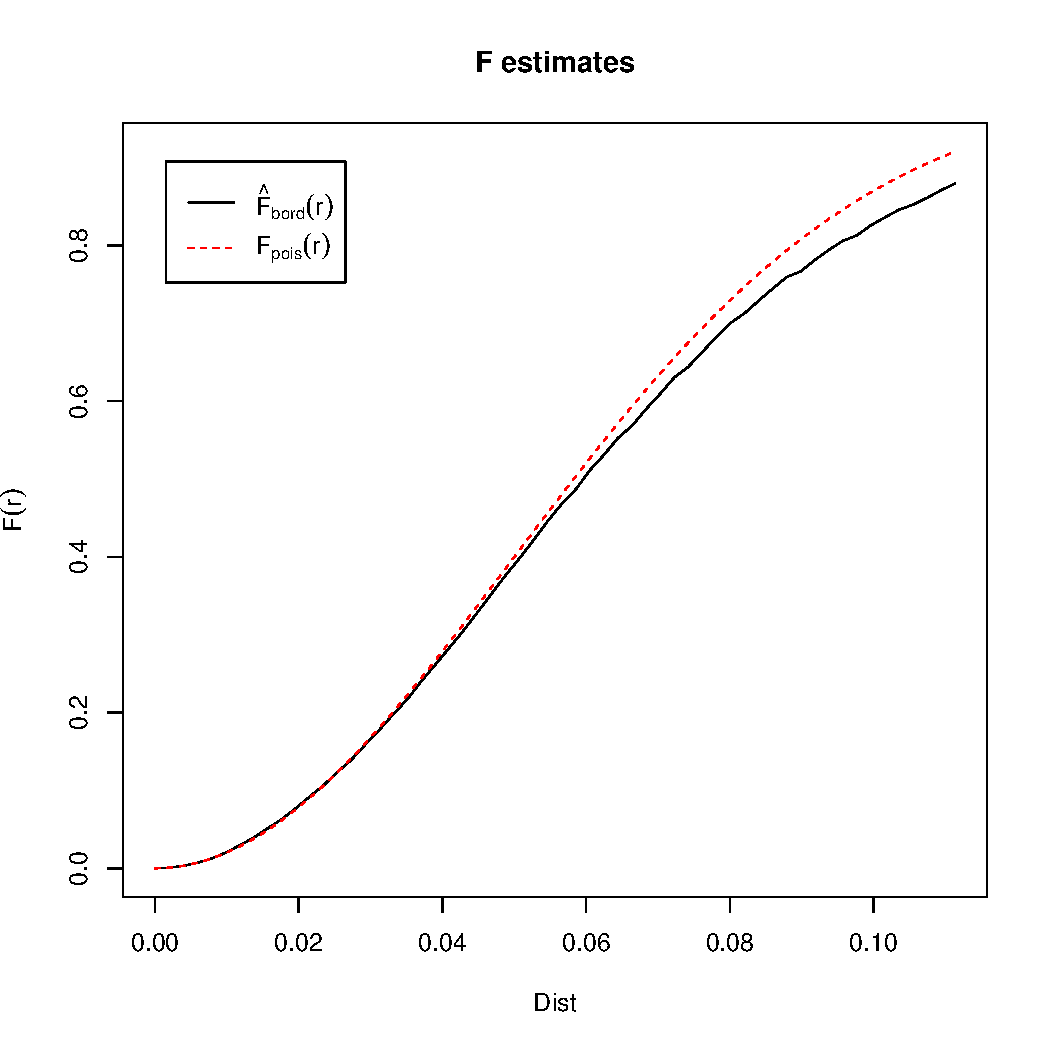
\includegraphics[width=\maxwidth]{figure/secondorder2} 
\begin{kframe}\begin{verbatim}
##      lty col  key           label                           meaning
## rs     1   1   rs hat(F)[bord](r) border corrected estimate of F(r)
## theo   2   2 theo      F[pois](r)          theoretical Poisson F(r)
\end{verbatim}
\end{kframe}
\end{knitrout}
\caption{Estimation of the G function using point-to-event distances and comparison with a theoretical poisson distribtion.}
\label{fest}
\end{figure}

\begin{figure}
\begin{knitrout}
\definecolor{shadecolor}{rgb}{0.969, 0.969, 0.969}\color{fgcolor}\begin{kframe}
\begin{alltt}
\hlstd{jp.khat}\hlkwb{<-}\hlkwd{Kest}\hlstd{(jp)}
\hlkwd{plot}\hlstd{(jp.khat,} \hlkwd{cbind}\hlstd{(border, theo)}\hlopt{~}\hlstd{r,} \hlkwc{main}\hlstd{=}\hlstr{"K function for JP data"}\hlstd{)}
\end{alltt}
\end{kframe}
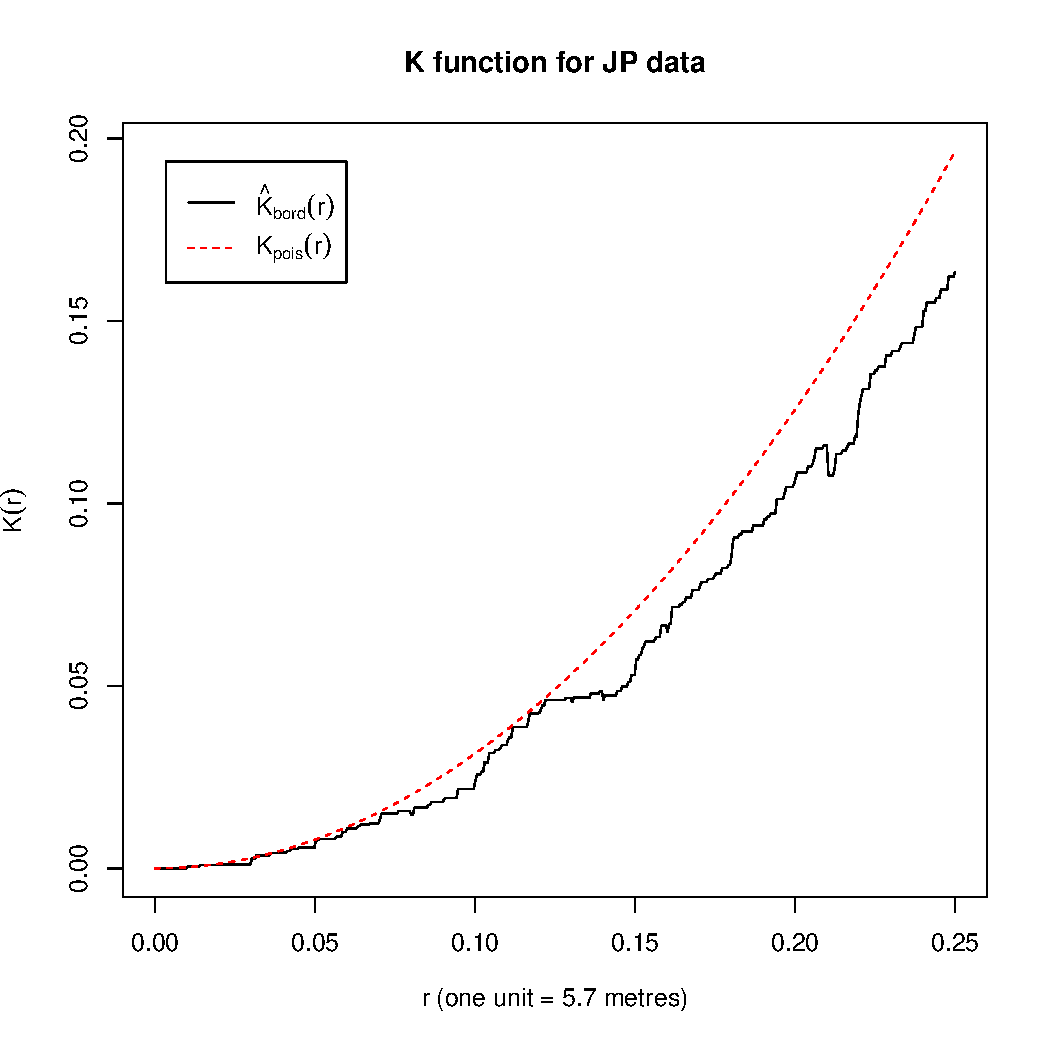
\includegraphics[width=\maxwidth]{figure/Kest} 
\begin{kframe}\begin{verbatim}
##        lty col    key           label                           meaning
## border   1   1 border hat(K)[bord](r) border-corrected estimate of K(r)
## theo     2   2   theo      K[pois](r)          theoretical Poisson K(r)
\end{verbatim}
\end{kframe}
\end{knitrout}
\caption{Plot of the K function for the japanese pine data showing the same pattern as the $\hat{G}$ and $\hat{F}$ plots.}
\label{kest}
\end{figure}

\begin{figure}
\begin{knitrout}
\definecolor{shadecolor}{rgb}{0.969, 0.969, 0.969}\color{fgcolor}\begin{kframe}
\begin{alltt}
\hlkwd{plot}\hlstd{(jp.khat,} \hlkwd{sqrt}\hlstd{(}\hlkwd{cbind}\hlstd{(border, theo)}\hlopt{/}\hlstd{pi)}\hlopt{-}\hlstd{r}\hlopt{~}\hlstd{r,}\hlkwc{ylab}\hlstd{=}\hlstr{"L(r)"}\hlstd{,} \hlkwc{main}\hlstd{=}\hlstr{"L function for jp"}\hlstd{,} \hlkwc{ylim}\hlstd{=}\hlkwd{c}\hlstd{(}\hlopt{-}\hlnum{0.025}\hlstd{,} \hlnum{0.025}\hlstd{))}
\end{alltt}
\end{kframe}
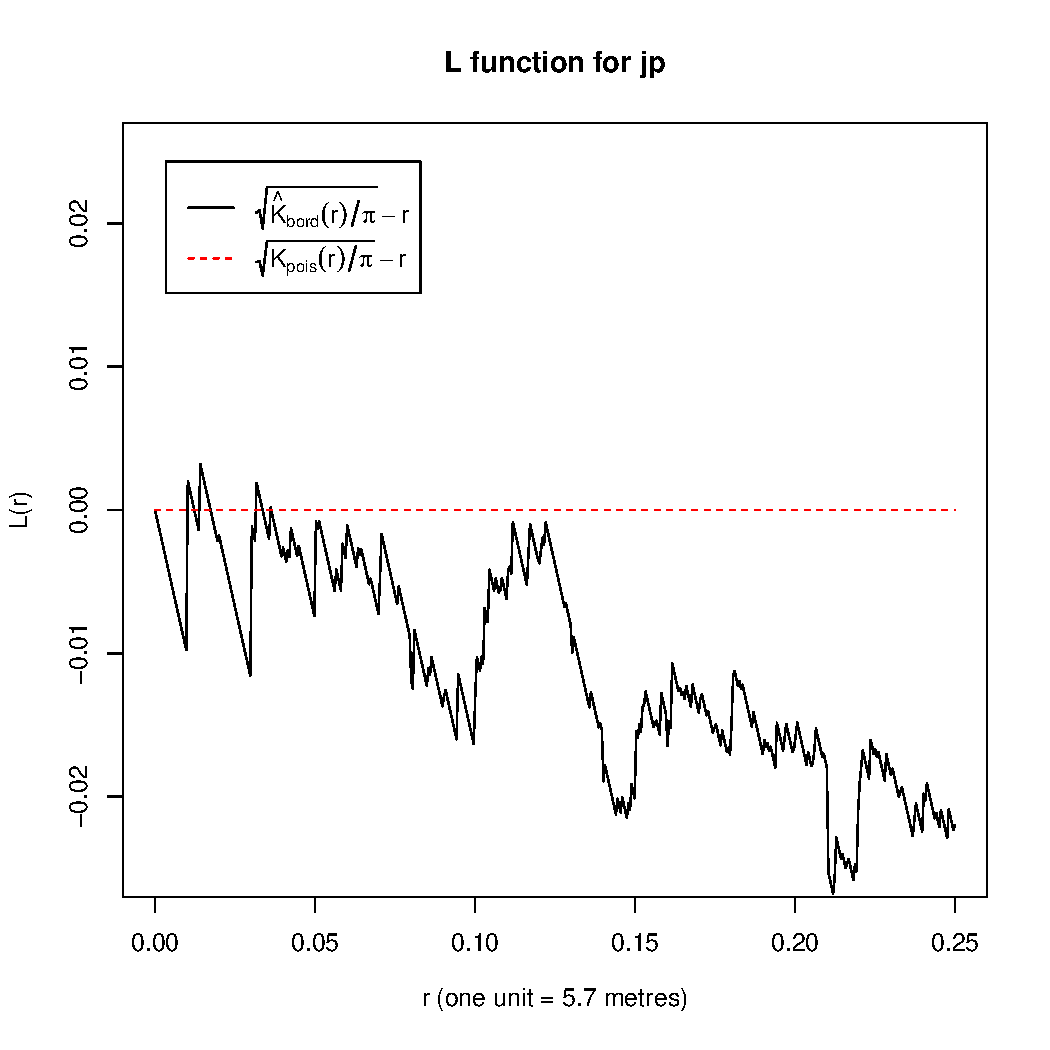
\includegraphics[width=\maxwidth]{figure/Lhat} 
\begin{kframe}\begin{verbatim}
##        lty col    key                      label
## border   1   1 border sqrt(hat(K)[bord](r)/pi)-r
## theo     2   2   theo      sqrt(K[pois](r)/pi)-r
##                                  meaning
## border border-corrected estimate of K(r)
## theo            theoretical Poisson K(r)
\end{verbatim}
\end{kframe}
\end{knitrout}
\caption{The $\hat{L}$ plot of the same japanses pine data suggesting a regular pattern in the data.}
\label{lest}
\end{figure}
\end{document}
